\section{Métricas de desarrollo de software}

Las métricas de software se pueden utilizar en modelos de predicción de fallas para mejorar la calidad del software al predecir la ubicación de la falla. En \cite{RADJENOVIC20131397} se realiza un análisis sistemático de la literatura desde 1991 hasta 2011. Entre los resultados destaca que las métricas orientadas a objetos (49\%) se utilizaron casi el doble de veces en comparación con las métricas de código fuente tradicionales (27\%) o las métricas de proceso (24\%). Las métricas orientadas a objetos de Chidamber y Kemerer (CK) fueron las más utilizadas. Según los estudios seleccionados existen diferencias significativas entre las métricas utilizadas en el rendimiento de la predicción de fallos. Se ha informado que las métricas de procesos y orientadas a objetos tienen más éxito en la búsqueda de fallas en comparación con las métricas tradicionales de tamaño y complejidad. Las métricas de proceso parecen ser mejores para predecir fallas posteriores al lanzamiento en comparación con cualquier métrica de código estático.

A pesar de la existencia de una gran cantidad de métricas de código en \cite{SINGH2024101253} proponen tres nuevas métricas basadas en la complejidad, el acoplamiento y cohesión del conjunto de métricas del repositorio PROMISE. El repositorio PROMISE fue creado para abordar la falta de conjuntos de datos públicos accesibles y estandarizados que puedan ser utilizados para el entrenamiento \cite{sayyad_shirabad_promise_2005,Sayyad-Shirabad+Menzies:2005} y validación de modelos de predicción en ingeniería de software y es uno de los mas utilizado en la literatura consultada \cite{ARAR2016106,RATHI2023119806,sharma2023far,NEVENDRA2022116217,PANDEY2020113085,rathore2021software}.

El repositorio PROMISE contiene una amplia gama de métricas de software que se utilizan para diversas investigaciones en ingeniería de software, particularmente en estudios de predicción de defectos y estimación de esfuerzos. Aunque el contenido exacto puede variar con las actualizaciones del repositorio y la inclusión de nuevos conjuntos de datos, típicamente incluye los siguientes tipos de métricas \cite{singh2024improved}:

\section*{Métricas de Código Fuente}
\begin{itemize}
  \item \textbf{Líneas de Código (LOC)}: Total de líneas de código, incluyendo líneas en blanco y comentarios.
  \item \textbf{Complejidad Ciclomática}: Mide la complejidad del código basándose en el número de caminos independientes a través del código.
  \item \textbf{Halstead Metrics}: Incluye esfuerzos calculados, volumen y dificultad, que son derivados del número de operadores y operandos únicos y totales en el código.
  \item \textbf{Número de Métodos por Clase (NOM)}: Cuantifica el número de métodos en cada clase.
  \item \textbf{Profundidad del Árbol de Herencia (DIT)}: Mide la profundidad de una clase en la jerarquía de herencia.
  \item \textbf{Número de Hijos (NOC)}: Contabiliza el número de clases directamente derivadas de una clase.
\end{itemize}

\section*{Métricas de Defectos}
\begin{itemize}
  \item \textbf{Defectos Reportados}: Número de defectos reportados para clases o módulos específicos.
  \item \textbf{Defect Density}: Densidad de defectos en relación con el tamaño del código.
\end{itemize}

\section*{Métricas de Proceso}
\begin{itemize}
  \item \textbf{Churn de Código}: Cambios en las líneas de código entre versiones sucesivas.
  \item \textbf{Frecuencia de Commits}: Número de commits realizados en un archivo o módulo.
  \item \textbf{Edad del Código}: Tiempo transcurrido desde la última modificación significativa.
\end{itemize}

\section*{Métricas de Diseño}
\begin{itemize}
  \item \textbf{Acomplamiento Entre Objetos (CBO)}: Mide el grado de interdependencia entre clases.
  \item \textbf{Aferent Couplings (Ca)} y \textbf{Eferent Couplings (Ce)}: Número de clases que dependen de una clase específica y número de clases de las cuales depende una clase específica, respectivamente.
  \item \textbf{Instability}: Proporción de Ce sobre la suma de Ca y Ce, indicando la estabilidad de una clase.
\end{itemize}

\section*{Métricas de Reutilización}
\begin{itemize}
  \item {Número de veces que una clase o función ha sido reutilizada en diferentes proyectos.
\end{itemize}

En \cite{PANDEY2021114595} realizan una revisión de la literatura de varios estudios desde 1990 hasta junio de 2019 sobre la aplicación del aprendizaje automático y el método estadístico sobre la predicción de fallas de software.


Indican que las métricas Orientadas a Objetos (OO) son más propensas a errores. Considerando que las métricas que se han empleado ampliamente son más funcionales en SFP. En la Fig. 7 podemos ver que LOC es la métrica más útil entre todas las métricas de OO, seguida por CBO

\begin{figure}[h!]
    \centering
    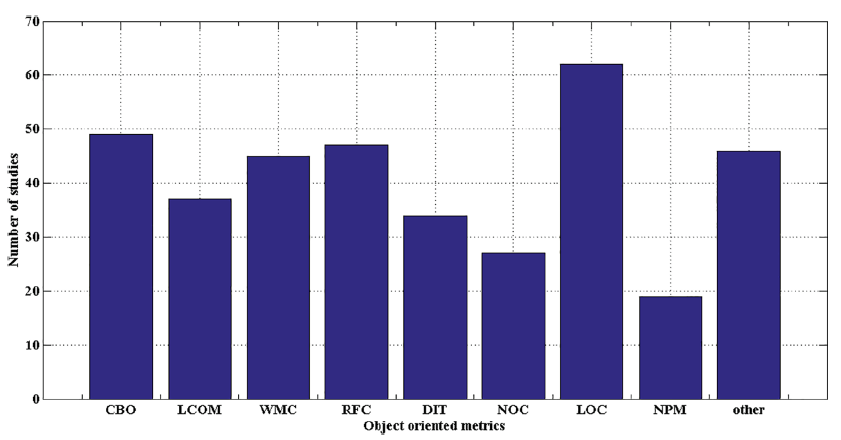
\includegraphics[width=\textwidth]{chapters/ChapterMarcoTeorico/sections/SoftwareMetrics/fig/oometrics.png}
    \setstretch{1} %Interlineado 1
	\captionsetup{labelsep=period, labelfont=bf}
    \caption{Lista de métricas de software orientado a objetos que son útiles para SFP. Tomado desde \cite{PANDEY2021114595}}
    \label{fig:OOmetrics}
\end{figure}